\subsection{The Hausdorff completion of a Noetherian ring}

Let A be a commutative ring, m an ideal of A and E an A-module; let \(\hat{A}\) and \(\hat{E}\) denote the respective Hausdorff completions of A and E with respect to the m-adic topology and \(j_{E}\) the canonical mapping \(E \rightarrow \hat{E}\) . The A-bilinear mapping \((a, x) \mapsto aj_{\mathrm{E}}(x)\) of \(\hat{A} \times E\) to \(\hat{E}\) defines an A-linear mapping

\[
\alpha_ {\mathrm{E}} \colon \hat {\mathrm{A}} \otimes_ {\mathrm{A}} \mathrm{E} \rightarrow \hat {\mathrm{E}},
\]

called canonical. Let \(u: \mathrm{E} \to \mathrm{F}\) be an A-module homomorphism and let \(\hat{u}\colon \hat{\mathbf{E}}\to \hat{\mathbf{F}}\) be the mapping obtained by passing to the Hausdorff completions; for \(a\in \hat{\mathbf{A}},x\in \mathbf{E},\)

\[
\alpha_ {\mathrm{F}} (a \otimes u (x)) = a j _ {\mathrm{F}} (u (x)) = a \hat {u} (j _ {\mathrm{E}} (x)) = \hat {u} (\alpha_ {\mathrm{E}} (a \otimes x)),
\]

in other words, the diagram

\pandocbounded{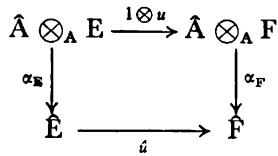
\includegraphics[keepaspectratio]{images/part002_24f0cc04.jpg}}

is commutative. Finally, it follows from § 2, no. 12, Proposition 16 that, if E is finitely generated, the homomorphism \(\alpha_{\mathbb{E}}\) is surjective.

THEOREM 3. Let A be a commutative Noetherian ring, m an ideal of A and E, F, G three finitely generated A-modules. Then:

\begin{enumerate}
\def\labelenumi{(\roman{enumi})}
\item
  If \(E \xrightarrow{u} F \xrightarrow{v} G\) is an exact sequence of A-linear mappings, the sequence \(\hat{E} \xrightarrow{\hat{u}} \hat{F} \xrightarrow{\hat{v}} \hat{G}\) obtained by passing to the Hausdorff completions (with respect to the m-adic topologies) is exact.
\item
  The canonical \(\hat{\mathbf{A}}\) -linear mapping \(\alpha_{\mathbf{E}}: \hat{\mathbf{A}} \otimes_{\mathbf{A}} \mathbf{E} \to \hat{\mathbf{E}}\) is bijective.
\item
  The A-module \(\hat{\mathbf{A}}\) is flat.
\end{enumerate}

We have seen that u and v are strict morphisms of topological groups (no. 2, Corollary to Theorem 2). Assertion (i) then follows from § 2, no. 12, Lemma 2. Assertion (ii) is obvious when E = A and the case where E is a free finitely generated A-module can be immediately reduced to that. In the general case, E admits a finite presentation

\[
\mathrm{L} \xrightarrow {u} \mathrm{L} ^ {\prime} \xrightarrow {v} \mathrm{E} \longrightarrow 0
\]

(Chapter I, § 2, no. 8, Lemma 8). We derive a commutative diagram

\pandocbounded{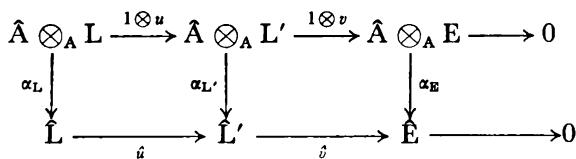
\includegraphics[keepaspectratio]{images/part002_14bc27b3.jpg}}

The first row is exact (Chapter I, § 2, no. 1, Lemma 1) and so is the second by (i). We already know that \(\alpha_{\mathrm{E}}\) is surjective (§ 2, no. 12, Proposition 16); on the other hand, as \(\alpha_{\mathrm{L}}\) and \(\alpha_{\mathrm{L}'}\) are bijective and \(1 \otimes v\) is surjective, \(\alpha_{\mathrm{E}}\) is injective by virtue of Chapter I, § 1, no. 4, Corollary 2 to Proposition 2; this shows (ii).

Then it follows from (i) and (ii) that, if \(a\) is an ideal of \(A\) (necessarily finitely generated), the canonical mapping \(\hat{A} \otimes_{A} a \to \hat{A}\) is injective, being the composition of \(\hat{a} \to \hat{A}\) and \(\alpha_{E}\) , which proves that \(\hat{A}\) is a flat A-module (Chapter I, § 2, no. 3, Proposition 1).

Under the conditions of Theorem 3 \(\hat{\mathbf{A}}\otimes_{\mathbf{A}}\mathbf{E}\) is often identified with \(\hat{\mathbf{E}}\) by means of the canonical mapping \(\alpha_{\mathbf{E}}\) . If \(u\colon \mathbf{E}\to \mathbf{F}\) is a homomorphism of finitely generated A-modules, \(\hat{u}\colon \hat{\mathbf{E}}\to \hat{\mathbf{F}}\) is then identified with \(1\otimes u\) by virtue of the commutativity of diagram (4).

COROLLARY 1. Let A be a commutative Noetherian ring, m an ideal of A, E a finitely generated A-module and F and G two submodules of E. Let A, E, F, G be given the m-adic topologies and let i be the canonical mapping from E to Ê. Then:

\[
\begin{array}{r l} \hat {\mathbf {F}} = \hat {\mathbf {A}}. i (\mathbf {F}), & (\mathbf {F} + \mathbf {G}) ^ {\wedge} = \hat {\mathbf {F}} + \hat {\mathbf {G}}, \\ & (\mathbf {F} \cap \mathbf {G}) ^ {\wedge} = \hat {\mathbf {F}} \cap \hat {\mathbf {G}}, \\ & (\mathbf {F}: \mathbf {G}) ^ {\wedge} = \hat {\mathbf {F}}: \hat {\mathbf {G}}. \end{array}
\]

Moreover, if a and b are two ideals of A and c = ab, \(\hat{c} = \hat{ab}\) .

By Theorem 3, \(\hat{\mathbf{E}}\) , \(\hat{\mathbf{F}}\) , \(\hat{\mathbf{G}}\) are canonically identified with \(\hat{\mathbf{A}} \otimes_{\mathbf{A}} \mathbf{E}\) , \(\hat{\mathbf{A}} \otimes_{\mathbf{A}} \mathbf{F}\) , \(\hat{\mathbf{A}} \otimes_{\mathbf{A}} \mathbf{G}\) , which establishes the first two formulae. The third and fourth follow respectively from Chapter I, § 2, no. 6, Proposition 6 and no. 10, Proposition 12. Finally, as \(\hat{\mathbf{a}} = \hat{\mathbf{A}}i(\mathfrak{a})\) , \(\hat{\mathfrak{b}} = \hat{\mathbf{A}}i(\mathfrak{b})\) , \(\hat{\mathfrak{c}} = \hat{\mathbf{A}}i(\mathfrak{c})\) ,

\[
\hat {\mathfrak {c}} = \hat {\mathrm{A}} i (\mathfrak {a b}) = \hat {\mathrm{A}} i (\mathfrak {a}) i (\mathfrak {b}) = \hat {\mathfrak {a b}}.
\]

COROLLARY 2. Let A be a commutative Noetherian ring, m an ideal of A and \(\hat{\mathbf{A}}\) the Hausdorff completion of A with respect to the m-adic topology. If an element \(a \in \mathbf{A}\) is not a divisor of 0 in A, its canonical image \(a'\) in \(\hat{\mathbf{A}}\) is not a divisor of 0 in \(\hat{\mathbf{A}}\) .

As \(\hat{\mathbf{A}}\) is a flat A-module, the corollary is a special case of Chapter I, § 2, no. 4, Proposition 3 (i).

COROLLARY 3. If A is a commutative Noetherian ring, the ring of formal power series A{[}{[}X₁, \ldots, Xₙ{]}{]} is a flat A-module.

It is the completion of the polynomial ring

\[
\mathbf {B} = \mathbf {A} [ \mathbf {X} _ {1}, \dots , \mathbf {X} _ {n} ]
\]

with respect to the m-adic topology, where m is the set of polynomials with no constant term (§ 2, no. 12, Example 1); as B is Noetherian (§ 2, no. 10, Corollary 2 to Theorem 2), A{[}{[}X₁, \ldots, Xₙ{]}{]} is a flat B-module by Theorem 3 and, as B is free A-module, A{[}{[}X₁, \ldots, Xₙ{]}{]} is a flat A-module (Chapter I, § 2, no. 7, Corollary 3 to Proposition 8).

PROPOSITION 8. Let A be a commutative Noetherian ring, m an ideal of A, \(\hat{A}\) the Hausdorff completion of A with respect to the m-adic topology and j the canonical mapping from A to \(\hat{A}\) . The :

\begin{enumerate}
\def\labelenumi{(\roman{enumi})}
\item
  \(\hat{\mathbf{A}}\) is a Zariski ring and \(\hat{\mathfrak{m}} = \hat{\mathbf{A}}.j(\mathfrak{m})\) is a defining ideal of \(\hat{\mathbf{A}}\) .
\item
  The mapping \(\mathfrak{n} \mapsto \hat{\mathfrak{n}} = \hat{\mathbf{A}}.j(\mathfrak{n})\) is a bijection of the set of maximal ideals of \(\mathbf{A}\) containing \(\mathfrak{m}\) onto the set of maximal ideals of \(\hat{\mathbf{A}}\) and \(\mathfrak{q} \mapsto j^{-1}(\mathfrak{q})\) is the inverse bijection.
\item
  Let \(\mathfrak{n}\) be a maximal ideal of \(\mathbf{A}\) containing \(\mathfrak{m}\) . The homomorphism \(j': \mathbf{A}_{\mathfrak{n}} \to \hat{\mathbf{A}}_{\hat{\mathfrak{n}}}\) derived from \(j\) is injective; if \(\mathbf{A}_{\mathfrak{n}}\) is identified by means of \(j\) with a subring of \(\hat{\mathbf{A}}_{\hat{\mathfrak{n}}}\) , the \((\mathfrak{n}\mathbf{A}_{\mathfrak{n}})\) -adic topology on \(\mathbf{A}_{\mathfrak{n}}\) is induced by the \(\hat{\mathfrak{n}}\) -adic topology on \(\hat{\mathbf{A}}_{\hat{\mathfrak{n}}}\) and \(\mathbf{A}_{\mathfrak{n}}\) is dense in \(\hat{\mathbf{A}}_{\hat{\mathfrak{n}}}\) with the \(\hat{\mathfrak{n}}\) -adic topology.
\end{enumerate}

Let us show (i). As \(\mathfrak{m}\) is a finitely generated ideal, \((\mathfrak{m}^n)^{\circ} = (\hat{\mathfrak{m}})^n = \mathfrak{m}^n\hat{\mathbf{A}}\) (§ 2, no. 12, Corollary 2 to Proposition 16) and the topology on \(\hat{\mathbf{A}}\) is the \(\hat{\mathfrak{m}}\) -adic topology. As \(\hat{\mathbf{A}}/\hat{\mathfrak{m}}\) is isomorphic to \(\mathbf{A}/\mathfrak{m}\) , it is a Noetherian ring and \(\hat{\mathfrak{m}} = \mathfrak{m}\hat{\mathbf{A}}\) is a finitely generated \(\hat{\mathbf{A}}\) -module and therefore \(\hat{\mathbf{A}}\) is Noetherian (§ 2, no. 10, Corollary 5 to Theorem 2); finally, as \(\hat{\mathbf{A}}\) is Hausdorff and complete with respect to the \(\hat{\mathfrak{m}}\) -adic topology, \(\hat{\mathbf{A}}\) is a Zariski ring (no. 3, Example 1).

Assertion (ii) follows immediately from the fact that the canonical homomorphism \(A/m \rightarrow \hat{A}/\hat{m}\) derived from j is bijective and the fact that every maximal ideal of \(\hat{A}\) contains \(\hat{m}\) , since \(\hat{A}\) is a Zariski ring and the Jacobson radical of \(\hat{A}\) then contains \(\hat{m}\) (no. 3, Proposition 6).

Finally let us prove (iii). As \(\mathfrak{n} = j^{-1}(\hat{\mathfrak{n}}), j(\mathbf{A} - \mathfrak{n}) \subset \hat{\mathbf{A}} - \hat{\mathfrak{n}}\) and \(j\) certainly defines a homomorphism \(j' \colon \mathbf{A}_{\mathfrak{n}} \to \hat{\mathbf{A}}_{\hat{\mathfrak{n}}}\) (Chapter II, § 2, no. 1, Proposition 2). Let us show that \(j'\) is injective; let \(a \in \mathbf{A}, s \in \mathbf{A} - \mathfrak{n}\) be such that

\[
j ^ {\prime} (a / s) = j (a) / j (s) = 0;
\]

then there exists \(s' \in \hat{\mathbf{A}} - \hat{\mathfrak{n}}\) such that \(s'j(a) = 0\) (Chapter II, §2, no. 1, Remark 3) and the annihilator of \(j(a)\) in \(\hat{\mathbf{A}}\) is therefore not contained in \(\hat{\mathfrak{n}}\) . Now, if \(\mathfrak{b}\) is the annihilator of \(a\) in \(\mathbf{A}\) , the annihilator of \(j(a)\) in \(\hat{\mathbf{A}}\) is \(\mathfrak{b}\) (Corollary 1 to Theorem 3); hence \(\mathfrak{b} \not\subset \mathfrak{n}\) , which shows that \(a / s = 0\) .

Moreover, there is a commutative diagram

\[
\begin{array}{c} \mathrm{A} / \mathfrak {n} ^ {k} \longrightarrow \mathrm{A} _ {\mathfrak {n}} / (\mathfrak {n} \mathrm{A} _ {\mathfrak {n}}) ^ {k} \\ \stackrel {{h}} {{\downarrow}} \qquad \qquad \qquad \qquad \qquad \qquad \qquad \qquad \qquad \qquad \qquad \qquad \qquad \qquad \qquad \qquad \qquad \qquad \qquad \qquad \qquad \qquad \qquad \hat {\mathrm{A}} / \hat {\mathfrak {n}} ^ {k} \longrightarrow \hat {\mathrm{A}} _ {\hat {\mathfrak {n}}} / (\hat {\mathfrak {n}} \hat {\mathrm{A}} _ {\hat {\mathfrak {n}}}) ^ {k} \end{array}\tag{5}
\]

where \(h\) and \(h'\) are derived from \(j\) and \(j'\) respectively and the horizontal arrows are the canonical isomorphisms of Chapter II, § 3, no. 3, Proposition 9. As \(n^k\) is an open ideal of A (since it contains \(m^k\) ), \(h\) is bijective and hence so is \(h'\) . This shows first that \((\mathfrak{n}\mathbf{A}_{\mathfrak{n}})^k = j'((\hat{\mathfrak{n}}\hat{\mathbf{A}}_{\hat{\mathfrak{n}}})^k)\) and hence the topology on \(\mathbf{A}_{\mathfrak{n}}\) is induced by that on \(\hat{\mathbf{A}}_{\hat{\mathfrak{n}}}\) ; moreover, \(\hat{\mathbf{A}}_{\hat{\mathfrak{n}}} = \mathbf{A}_{\mathfrak{n}} + (\hat{\mathfrak{n}}\hat{\mathbf{A}}_{\hat{\mathfrak{n}}})^k\) for all \(k > 0\) and hence \(\mathbf{A}_{\mathfrak{n}}\) is everywhere dense in \(\hat{\mathbf{A}}_{\hat{\mathfrak{n}}}\) .

COROLLARY. Let A be a Noetherian local (resp. semi-local) ring and m its Jacobson radical. Then \(\hat{A}\) is a Noetherian local (resp. semi-local) ring whose Jacobson radical is \(\hat{m}\) .

\(\hat{\mathbf{A}}\) is Noetherian by Proposition 8 (i) and the rest follows from Proposition 8 (ii) and the third formula in Corollary 1 to Theorem 3.

